\section{Plugins}
\label{sec:plugins}

%Coisas importantes para discutirmos:
%\begin{itemize}
%  \item \C{GST_STATIC_PAD_TEMPLATE} - OK
%  \item \C{gst_my_filter_class_init} - OK
%  \item \C{gst_myfilter_init} - OK
%  \item \C{myfilter_chain} - OK
%  \item \C{myfilter_plugin_init} - OK
%  \item \C{GST_PLUGIN_DEFINE} - OK
%  \item Definição de propriedades?
%  \item Eventos?
%\end{itemize}

Até agora só vimos como usar elementos já definidos pelo Gstreamer (e.g.
``filesrc'', ``alsasink'').  Nesta seção iremos discutir de forma introdutória
como é possível criar novos tipos de elementos.  O objetivo nesta seção não é
detalhar cada uma das funções/classes do GStreamer que permitem que ele seja
estendido~(para isso existe o manual e documentação do código GStreamer), mas
sim permitir, a partir da discussão de dois exemplos concretos, que o
leitor possa ter uma visão geral de como desenvolver novos elementos.  A
prática de desenvolvê-los irá nos permitir identificar as principais funções
que devem ser implementadas por um novo elemento do Gstreamer e como
encapsulá-lo em um plugin.  Na prática, entretanto, para desenvolver elementos
complexos, o leitor provavelmente também necessitará consultar o manual do
GStreamer, e possivelmente também o seu código.

\subsection*{Elemento ``myfilter''}
No Gstreamer, novos tipos de elementos podem ser criados estendendo a classe
base \C{GstElement}.  Também é possível encapsular esses novos elementos em
plugins que podem ser distribuídos separadamente, instalados e carregados
dinamicamente.  Para entendermos como desenvolver um novo elemento para o
GStreamer, iremos começar com um exemplo simples (que chamaremos de
``myfilter'') que ao receber algum dado no seu \en{sink pad} irá apenas
imprimir o tamanho do buffer recebido e retransmitir esses dados em seu
\en{source pad}.  O código fonte do nosso novo elemento ``myfilter'' está
divido em dois arquivo (\C{myfilter.h} e \C{myfilter.c}) e será detalhado a
seguir.

O arquivo \C{myfilter.h} (Listagem~\ref{lst:myfilter_h}) declara uma classe que
representa o novo tipo de elemento que queremos criar (\C{GstMyFilter}).  A
definição dessa classe segue o padrão do \emph{framework} GObject, e deve
estender a classe \C{GstElement} (definida no arquivo \C{gst/gst.h}).  Por
isso, é necessário criar as estruturas \C{_GstMyFilter}~(linhas 6--9) e
\C{_GstMyFilterClass}~(linhas 11--13).  A classe \C{GstMyFilter} deve estender
a classe \C{GstElement}---por isso a estrutura \C{_GstMyFilter} define o campo
\C{element} do tipo \C{GstElement}, linha 7, e a estrutura
\C{_GstMyFilterClass} define o campo \C{parent_class} do tipo
\C{GstElementClass}, linha 12.  As linhas 15--24 definem macros padrões que
usam o \en{framework} GObject para checagem e \en{casting} do novo tipo
definido.  Por fim, a função \C{get_my_filter_get_type}, declarada na linha 26,
é requerida pelo \en{framework} GObject para criar novas instâncias da 
classe \C{GstMyFilter}.

\lstinputlisting[
style=display,
caption={Arquivo myfilter.h},
label={lst:myfilter_h},
]{src/myfilter.h}

O arquivo \C{myfilter.c}~(Listagem~\ref{lst:myfilter_c}) implementa as funções
que permitem ao GStreamer carregar instâncias deste novo elemento e utilizá-las
em \en{pipeline}s, bem como a lógica do processamento realizado por esse
elemento.  A principais funções são as funções de inicialização (\C{*_init}) e
a de processamento (\C{*_chain}). A Tabela~\ref{tab:funcs} descreve brevemente
essas funções.

\begin{table}
  \centering
  \begin{tabular}{ | l | c |}
    \hline
    Função         & Descrição \\ \hline\hline
    *\_class\_init & Inicializa uma classe \\ \hline
    *\_init        & Inicializa uma instância de uma classe \\ \hline
    *\_chain       & Chamada quando há novos \textit{buffers} no 
                      \textit{sink pad} \\ \hline
  \end{tabular}
  \caption{Principais funções para definição de um novo elemento.}
  \label{tab:funcs}
\end{table}

%Rodrigo: Acho que esse parágrafo podia sair ou deixar apenas a primeira frase
%         dele. Não sei se precisa entrar em tantos detalhes dessa função.%
A função \C{gst_my_filter_class_init}~(linhas 30--48) é chamada na primeira vez
que um objeto do tipo \C{GstMyFilter} for instanciado.  Essa função define
metadados para a classe, por meio do método \C{gst_class_set_static_metadata},
e define os tipos de \en{pads} do novo elemento que estamos criando, através
das chamadas \C{gst_element_class_add_pad_template}.  As chamadas dessa função
utilizam os dados de duas estruturas do tipo \C{GstStaticPadTemplate}
(respectivamente, \C{sink_factory} e \C{src_factory}, linhas 6--16).  A macro
\C{GST_STATIC_PAD_TEMPLATE} ajuda a preencher os valores dos campos de
estruturas \C{GstStaticPadTemplate}.  Ela recebe como parâmetros: (1)~um nome
para o \en{pad}; a direção do \en{pad} (\C{GST_PAD_UNKNOWN},
\C{GST_PAD_SRC} ou \C{GST_PAD_SINK}); a sua informação de presença
(\C{GST_PAD_ALWAYS}, \C{GST_PAD_SOMETIMES} ou \C{GST_PAD_REQUEST}); e as
capacidades do \en{pad}, uma estrutura do tipo \C{GstCaps *}.  Geralmente, a
inicialização de uma estrutura do tipo \C{GstCaps} é feita por meio da macro
\C{GST_STATIC_CAPS}.  No nosso exemplo, linhas 10 e 16, tanto a \en{sink pad}
como a \en{src pad} do elemento que estamos criando recebe qualquer tipo de
dado (por isso, o parâmetro \C{"ANY"}.
%Como mencionado anteriormente, cada elemento do pipeline pode ter zero ou mais
%\emph{source pads} e zero ou mais \emph{sink pads}.  O número de \emph{pads} e
%quais são esses \emph{pads} podem ser definidos estaticamente ou dinamicamente.
%No nosso exemplo, queremos um elemento que tenha apenas um \emph{source} e um
%\emph{sink pad}.  Por isso, a definição dos \emph{pads} desse elemento é feita
%de forma estática.

A função \C{gst_my_filter_init}~(linhas 50--61) é chamada quando uma nova
instância da classe \C{GstMyFilter} é criada.  Ela basicamente cria as
instâncias da classe \C{GstPad} relacionadas a cada um dos \en{pads} do
elemento \C{GstMyFilter}, chamadas \C{gst_pad_new_from_static_template} (linhas
53 e 58).  Além disso, é também na função \C{gst_my_filter_init}, por meio da
função \C{gst_pad_set_chain_function}, que a função é registrada para ser
chamada sempre que novos dados apareçam no \en{sink pad} do elemento
``myfilter''.

A função \C{gst_my_filter_chain}~(linhas 18--27) é a função de fato responsável
por fazer o processamento de dados relacionado com o elemento que estamos
criando.  Essa função será chamada sempre que novos dados chegarem no
\en{sink pad} do nosso elemento.  Ela recebe um ponteiro para o \en{pad}
(\C{GstPad*}) onde os dados chegaram, um ponteiro para o pai (\C{GstObject*}) e
um ponteiro para o buffer de dados que está chegando por esse \en{pad}
(\C{GstBuffer *}).  No nosso exemplo, essa função apenas imprime o tamanho do
buffer recebido~(acessado por meio da chamada \C{gst_buffer_get_size(buf)}) e
reenvia esse buffer para o \en{src pad} do elemento (usando a chamada
\C{gst_pad_push}).

%A macro \C{G_DEFINE_TYPE}, linha 4, também faz parte do
%\emph{framework} GObject e expande para a declaração das funções de
%inicialização de classe (neste caso as funções \C{gst_my_filter_init} e
%\C{gst_my_filter_class_init}).  Além disso, esta macro também expande para 
%outras funções e variáveis úteis para o \emph{framework}, tais como
%\C{*_get_type()} e \C{*_parent_class}.

As linhas 70 a 78 trazem as definições relacionadas ao encapsulamento do nosso
novo elemento em um plugin.  A macro \C{GST_PLUGIN_DEFINE} é usada para
definir o ponto de entrada (a função que será chamada quando o plugin for
carregado pelo GStreamer) e metadados para um plugin.  A macro recebe a versão
do GStreamer que é compatível com o  plugin (dividido em \en{major} e
\en{minor}), o nome do plugin, uma descrição do plugin, um ponteiro para a
função de inicialização~(no nosso caso \C{my_filter_plugin_init}).  A função 
\C{my_filter_plugin_init} é chamada quando o GStreamer carrega o plugin.  No
nosso exemplo, ela apenas registra a classe \C{GstMyFilter}, por meio da função
\C{gst_element_register}, como um novo elemento do Gstreamer, o qual poderá ser
acessado pelo nome ``myfilter''.

\lstinputlisting[
style=display,
caption={Arquivo myfilter.c.},
label={lst:myfilter_c},
]{src/myfilter.c}

\subsection*{Compilando e testando o novo elemento (``myfilter'')}
Para compilar o nosso plugin devemos gerar uma biblioteca dinâmica (.dll no
Windows ou .so no Linux).  O comando a seguir compila o exemplo desenvolvido
acima, gerando o arquivo \C{myfilter.so}:

\begin{lstlisting}[style=command]
@\$@ cc -shared -fPIC \
  `pkg-config --cflags --libs gstreamer-1.0 gstreamer-base-1.0`\
  myfilter.c -o myfilter.so
\end{lstlisting}

Assumindo que o arquivo gerado \C{myfilter.so} esteja no caminho atual, é
possível, por exemplo, carregar o elemento ``myfilter'' que desenvolvemos em um
\emph{pipeline} simples através da ferramenta \C{gst-launch}:

\begin{lstlisting}[style=command]
@\$@ gst-launch-1.0 --gst-plugin-path=. \
     audiotestsrc !  myfilter ! alsasink
\end{lstlisting}

O parâmetro \C{--gst-plugin-path} está sendo usado aqui para informar que o
GStreamer também deve buscar plugins no diretório corrente da linha de comando.
Como o elemento que desenvolvemos recebe qualquer tipo de dado (tipo de \en{pad
sink} \C{ANY}, é possível utilizá-lo usá-lo em qualquer \en{pipeline}.  Por
exemplo, compare a execução do \en{pipeline} anterior com a execução seguinte
\en{pipeline}:

\begin{lstlisting}[style=command]
@\$@ gst-launch-1.0 --gst-plugin-path=. \
     videotestsrc ! myfilter ! ximagesink
\end{lstlisting}

\subsection*{Exemplo de um novo elemento para filtro de vídeo}
Como mencionado anteriormento, os elementos do Gstreamer são derivados da
classe base \en{GstElement}.  Porém, quando queremos desenvolver elementos mais
complexos pode ser interessante nos basearmos em outras classes distribuídas
nos pacotes \C{gst-plugin-base}.  A Figura~\ref{fig:plugins_base_classes}
evidencia algumas dessas classes e como elas estão relacionadas.

A classe \C{GstBaseSrc} é um classe base para plugins tipo \en{source} (ou
produtores).  A classe \C{GstBaseSink} é uma classe base para plugins do tipo
\en{sink} (ou consumidores).  A classe \C{GstBaseTransform} é uma classe base
para plugins do tipo \en{tranform} (ou filtros).  Além disso, quando estamos
tratando especificamente de áudio ou vídeo, as classes \C{GstAudioFilter} e
\C{GstVideoFilter} também podem ser interessantes para desenvolvermos novos
filtros.

\tikzstyle{every node}=[draw=black,thick,anchor=west,font=\scriptsize]
\tikzstyle{selected}=[draw=red,fill=red!30]
\tikzstyle{optional}=[dashed,fill=gray!50]
\begin{figure}[H]
  \centering
  \begin{tikzpicture}[%
  grow via three points={one child at (0.5,-0.7) and
  two children at (0.5,-0.7) and (0.5,-1.4)},
  edge from parent path={(\tikzparentnode.south) |- (\tikzchildnode.west)}]
  \node {GObject}
    child {
%      node {GInitiallyUnknown}
%      child {
        node {GstElement}
        child {node{GstBaseSrc}}
        child {node{GstBaseSink}}
%        child {node{GstBin}}
        child {
          node {GstBaseTransform}
          child {node {GstAudioFilter}}
          child {node {GstVideoFitter}}
        }
%      }
    };
  \end{tikzpicture}
  \label{fig:plugins_base_classes}
  \caption{Hierarquia de classes evidenciando algumas classes importantes no
           desenvolvimento de novos elementos para o GStreamer.}
\end{figure}

O nosso próximo exemplo---elemento ``myvideofilter''---irá usar a classe
\C{GstVideoFilter} para exemplificar como é possível criarmos um elemento que
processa frames de vídeo.  O objetivo do nosso filtro é aplicar um ``efeito de
onda'' no vídeo~(veja Figura~\ref{fig:bunny_myvideofilter}).  Nesse filtro,
cada pixel $(u, v)$ do frame original~(recebido no \en{sink pad} do elemento)
será mapeado para uma posição $(x, y)$ no frame de saída segundo a fórmula:
\begin{equation}
  \begin{cases}
  x(u, v) = u + 20 \times sin ( FACTOR \times v); \\
  y(u, v) = v;
  \end{cases}
  \label{eq:wave_filter}
\end{equation}
onde $FACTOR$ é uma propriedade (um valor real) cujo valor pode ser atribuído
após a instanciação do elemento.

Assim como o exemplo anterior, o elemento \en{myvideofilter} também está
dividido em dois arquivos: \C{myvideofilter.h} e \C{myvideofilter.c}.

O arquivo \C{myvideofilter.h} (Listagem~\ref{lst:myvideofilter_h}) é bastante
similar ao exemplo anterior e traz a declaração da classe \C{MyVideoFilter},
por meio das estruturas \C{GstMyVideoFilter} e \C{GstMyVideoFilterClass},
linhas 8--10 e 12--14, respectivamtente.  Diferente do exemplo anterior,
entretanto, essa classe estende a classe base \C{GstVideoFilter}.  A classe
\C{MyVideoFilter} também define um campo, \C{factor}, que guardará o valor do
parâmetro passado pelo usuário.

\lstinputlisting[
style=display,
caption={myvideofilter.h},
label={lst:myvideofilter_h},
]{src/myvideofilter.h}

O arquivo \C{myvideofilter.c}~(Listagem~\ref{lst:myvideofilter_c}) implementa
as principais funções da classe \C{MyVideoFilter}.  Comparado com o exemplo
anterior as principais diferenças são: as capacidades dos \en{pads}; a
definição da propriedade \C{factor}, a partir da qual o usuário pode controlar 
o efeito do filtro; e a função de transformação.

%Rodrigo: Eu dividiria as funções em listagens diferentes. Primeiro mostraria
%         só as *_init e depois, quando comentasse sobre propriedade,
%         mostraria o get e set. Mesmo vale pra função *_transform%
\lstinputlisting[
style=display,
caption={myvideofilter.c},
label={lst:myvideofilter_c},
]{src/myvideofilter.c}

Diferente do exemplo anterior, que recebia qualquer dado no seu \en{sink pad},
o elemento ``myvideofilter'' receberá como entrada frames de vídeo e produzirá
como saída também frames de vídeo.  Por isso, na definição dos templates das
capacidades, linhas 10--12, agora usamos a macro o \C{GST_VIDEO_CAPS_MAKE}.
Essa macro recebe uma string que descreve o leaiute dos pixels (e.g. ``I420'',
``RGB'', ``YV12'', ``YUY2'', ``AYUV'' etc.).  Para manter o exemplo o mais
simples possível, aqui estamos usando apenas ``BGRx'' e ''RGB'', linhas 14 e
21.

A definição das propriedades do elemento é feita baseada no \en{framework}
GObject, por isso a definição da enumeração, linhas 27--29, e das funções
\C{gst_my_video_filter_set_property} e \C{gst_myvideo_filter_get_property}.  Na
função de inicialização da classe \C{gst_my_video_filter_class_init} também
definimos que essas funções são chamadas para tratar alterações nessas
propriedades, linhas 121--122, e ``instalamos'' a propriedade por meio da
chamada \C{g_object_install_property}, linhas 125--130.  O GStreamer consulta
as propriedades definidas por meio do GObject para saber quais os parâmetros
que podem ser passados para o elemento.  Como mencionado anteriormente, é
possível consultar os parâmetros de um elemento por meio do comando
\C{gst-inspect}~(voltaremos à isso mais a frente).

Diferente da classe \C{GstElement}, que requer uma função de transformação que
trabalhe com um buffer arbitário~(\C{GstBuffer}), a classe \C{GstVideoFilter}
já permite que criemos uma função que recebe como entrada e produz como saída
frames de vídeo (\C{GstVideoFrame}s).  Para isso, temos que implementar a
função \C{transform_frame}.  No nosso caso, criamos a função
\C{gst_my_video_transform_frame}, linhas 64--97, e a registramos como a função
de transformação do frame de vídeo na 133.

A função \C{gst_my_video_transform} é de fato a mais importante do nosso exemplo.
É nessa função onde os pixels do frame de entrada são mapeados em suas posições
no frame de saída, conforme a Equação~\ref{eq:wave_filter}, linhas 83--94.
% Para podermos fazer isso aqui, usamos algumas macros do GStreamer, tais como
% \C{GST_VIDEO_FRAME_COM_WIDTH} e \C{GST_VIDEO_FRAME_COMP_HEIGHT}.  Alguns
% detalhes de como os pixels estão organizados no frame são necessários para
% podermos ``andar'' corretamente no frame e copiarmos os seus pixels para o
% frame de saída. 

Por fim, a definição do plugin e a função \C{gst_my_video_plugin_init} são bem
similares ao exemplo anterior e não necessitam de mais detalhes aqui.

\subsection*{Compilando e testando o elemento ``myvideofilter''}
Para compilar o element ``myvideofilter'' como um plugin é possível usar um
comando similar ao do exemplo anterior.  A única diferença é que agora estamos
nos baseando na classe base \C{GstVideoFilter} e, por isso, também temos que
incluir as flags de compilação e linkagem dos pacote \C{gstreamer-video-1.0}.

\begin{lstlisting}[style=command]
@\$@ cc -shared  -fPIC \
     `pkg-config --libs --cflags gstreamer-1.0 gstreamer-base-1.0 \
                                 gstreamer-video-1.0` \
     myvideofilter.c -o myvideofilter.so
\end{lstlisting}

Se tudo correr bem com o comando acima, o arquivo \C{myvideofilter.so} (ou .dll
no caso do sistema operacional Windows) será
gerado e já é possível usar elemento em \en{pipeline}s do GStreamer; como por
exemplo:

\begin{lstlisting}[style=command]
@\$@ gst-launch-1.0 --gst-plugin-path=. filesrc location=bunny.ogg ! \
     oggdemux ! theoradec ! videoconvert ! videoscale ! \
     video/x-raw,width=720 ! myvideofilter factor=0.10 ! ximagesink
\end{lstlisting}

Para verificarmos os detalhes do elemento que criamos, também podemos executar
o comando \C{gst-inspect}, e.g.: 
\begin{lstlisting}[style=command]
@\$@ gst-inspect-1.0 --gst-plugin-path=. myvideofilter
\end{lstlisting}
que imprimirá na tela:

\lstinputlisting[
style=display,
caption={Saída do programa gst-inpect-1.0, consultando os detalhes do elemento
         ``myvideofilter''.},
label={lst:myvideofilter_gstinspect},
]{src/myvideofilter.gstinspect}

A Figura~\ref{fig:bunny_myvideofilter} mostra exemplos de uso do filtro
``myvideofilter'' com diferentes valores para o parâmetro \en{factor}.

\begin{figure}[H]
  \centering
  \subfigure[factor=0.01]{
    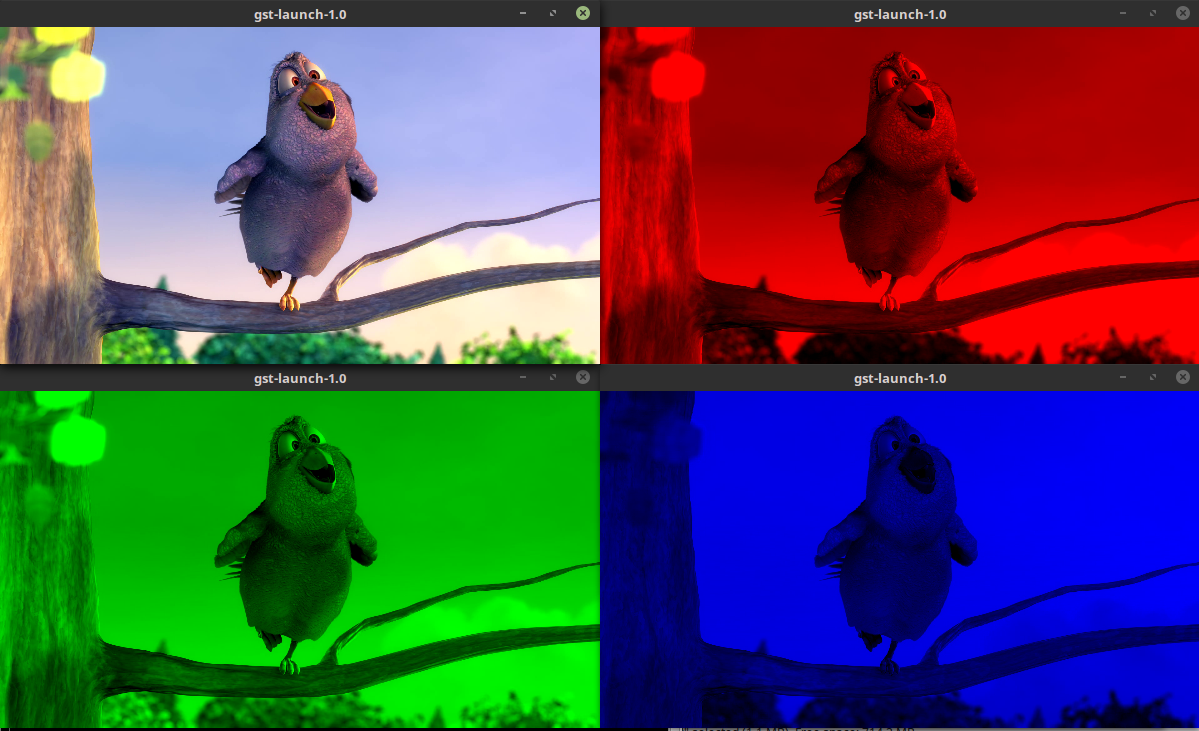
\includegraphics[width=0.4\textwidth]{pics/myvideofilter}
  }
  \subfigure[factor=0.05]{
    \includegraphics[width=0.4\textwidth]{pics/myvideofilter2}
  }
  \subfigure[factor=0.1]{
    \includegraphics[width=0.4\textwidth]{pics/myvideofilter3}
  }
  \caption{Exemplos da execução de pipelines usando o elemento
           ``myvideofilter''.}
  \label{fig:bunny_myvideofilter}
\end{figure}

